\documentclass{a0poster}
\usepackage{fancytikzposter} % here most of the things are defined
\usetemplate{4}
\usepackage[margin=\margin cm, paperwidth=84.1cm, paperheight=118.9cm]{geometry}
%\usepackage[margin=\margin cm, paperwidth=59.4cm, paperheight=84.0cm]{geometry}
\title{Imfact of Orange Peel Coupling \\ on Magnetization Switching in Nanopillar}
\author{D. Aravinthan$^*$ and M. Daniel \\Centre for Nonlinear Dynamics\\ School of Physics, Bharathidasan University\\ Tiruchirappalli - 620 024\\\texttt{}
\And
P. Sabareesan\\School of Electrical and Electronics Engineering\\ SASTRA University\\Thanjavur - 613 401}
\begin{document}
\AddToShipoutPicture{\BackgroundPicture}
\noindent
\begin{tikzpicture}
\initializesizeandshifts
\titleblock{100}{1.25}
%%%%%%%%%%%%%%%%%%%%%%%%%%%%%%%%%%%%%%%Block%%%%%%%%%%%%%%%%%%%%%%%%%%%%%%%%%%%%%%%%%%%%%%%%%%%%%%%%%%%%
\blocknode{Introduction}{
\large
\begin{itemize}
\item Recently magnetization switching in nanopillar devices has been a continuously growing topic, because of its potential applications in ultra-high density recording media, magnetic memory devices, magnetic sensors and read / write heads etc. 
\item The speed of switching of magnetization in magnetic trilayers is an issue of increasing importance for applications. Magnetocrystalline anisotropy, shape anisotropy and surface anisotropy play a vital role in reducing the switching time.
\item There is an important magnetostatic coupling between the ferromagnetic layers in the nanopillar  due to surface roughness  referred as \textbf{Neel Coupling} or \textbf{Orange Peel Coupling} which is expected to contribute to the reduction of the switching time.
\item In this work, we investigate the impact of orange peel coupling on magnetization switching time in  Co/ Cu/ NiFe (Py) nanopillar device. 
\end{itemize}
}
% Next Block%%%%%%%%%%%%%%%%%%%%%%%%%%%%%%%%%%%%%%%%%%%%%%%%%%%%%%%%%%%%%%%%%%%%%%%%%%%%%%%%%%%%%%%%%%%%%%%%%%
\blocknode{Geometry: Co/Cu/NiFe Nanopillar}{
\Large
\begin{tikzfigure}
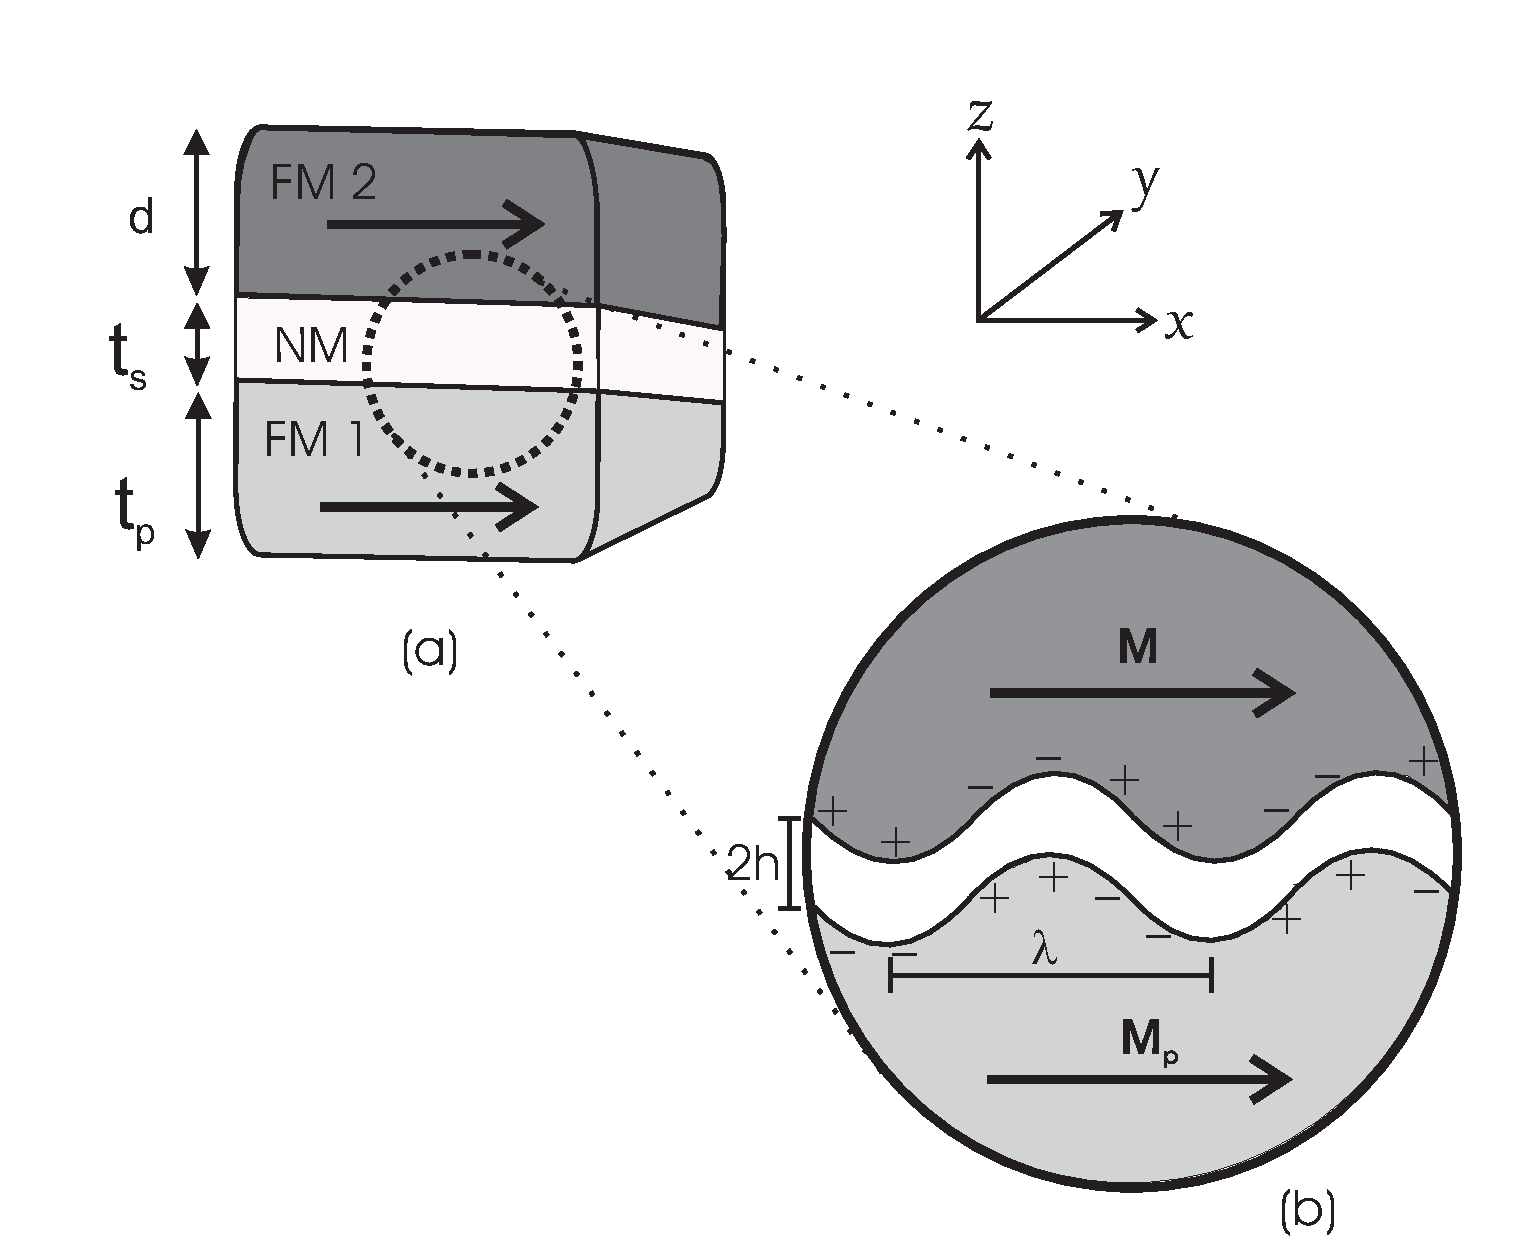
\includegraphics[width=5in]{opc_model}
\end{tikzfigure}
\begin{center}
{\large Fig.1: Schematic sketch of the Co/Cu/NiFe nanopillar device.}
\end{center}
}
%%%%%%%%%%%%%%%%%%%%%%%%%%%%%%%%%%%%%%%%%%%%%%%%%%%%%%%%%%%%%%%%%%%%%%%%%%%%%%%%%%%%%%%%%%%%%%%%%%%%%%%%%%%%%%
\blocknode{Magnetization Switching Dynamics}{
\large
\begin{itemize}
\item The magnetization switching  dynamics of the free layer is governed by the Landau-Lifshitz-Gilbert-Slonczewski(LLGS) equation
\begin{equation}
\frac{d\mathbf{M}}{dt}=-\gamma [\mathbf{M}\times \mathbf{H}_{eff}] -\frac{\alpha \gamma }{M_{s}}[\mathbf{M}\times(\mathbf{M}\times\mathbf{H}_{eff})]+\gamma a_{j}[\mathbf{M}\times(\mathbf{M}\times\mathbf{M}_{p})],
\label{llgs}
\end{equation}
~~~~~~~~~~~~~~~~~~~~~~~~~where, $a_{j}=\frac{pJ\hbar}{\mu_{0} edM_{s}^{2}}\cdot$
\end{itemize}
\innerblock{Effective field in the free layer}{
\begin{equation}
\mathbf{H}_{eff}= \mathbf{H}_{ma}+\mathbf{H}_{shape}+\mathbf{H}_{ext}+\mathbf{H}_{opc}
\label{eff}
\end{equation}
{\bf Magnetocrystalline Anisotropy}~~:~~$\mathbf{H}_{ma}=h_{a}M^{x}\mathbf{e}^{x}$, where, $h_{a}=\frac{2k_{a}}{\mu_{0}M_{s}^{2}}$ \\

{\bf Shape Anisotropy}~~~~~~~~~~~~~~~~~~~:~~$\mathbf{H}_{shape}= - [N_{x}M^{x}\mathbf{e}^{x}+N_{y}M^{y}\mathbf{e}^{y}+N_{z}M^{z}\mathbf{e}^{z}]$\\

{\bf External Magnetic Field}~~~~~~~~:~~$\mathbf{H}_{ext}=H_{e}\mathbf{e}^{y}$\\

{\bf Orange Peel Coupling Field}~~~~~:~~$\mathbf{H}_{opc}=h_{n}M^{y}\mathbf{e}^{y},$ where $h_{n}=\frac{\pi ^{2}h^{2}}{\sqrt{2}\lambda d} \exp\left(\frac{-2\sqrt{2}\pi t_{s}}{\lambda }\right)$\\

{\bf Total Effective Field}~~~~~~~~~~~~~~~~~:~~$\mathbf{H}_{eff}=h_{a}M^{x}\mathbf{e}^{x}-N_{z}M^{z}\mathbf{e}^{z}+H_{e}\mathbf{e}^{y}+h_{n}M^{y}\mathbf{e}^{y}.$\\
}
}
%%%%%%%%%%%%%%%%%%%%%%%%%%%%%%%%%%%%%%%%%%%%%%%%%%%%%%%%%%%%%%%%%%%%%%%%%%%%%%%%%%%%%%%%%%%%%%%%%%%%%%%%%%%%%%
\blocknode{Numerical Results}{
\large
The dimensionless LLGS equation is
\begin{align}
\displaystyle
\label{dllgs}
& \frac{d\mathbf{m}}{d\tau }=-[\mathbf{m}\times \left(h_{a}m^{x}\mathbf{e}^{x}+(h_{e}+h_{n}m^{y})\mathbf{e}^{y}-N_{z}m^{z}\mathbf{e}^{z}\right)] \\ \nonumber
&-\alpha[\mathbf{m}\times(\mathbf{m}\times \left(h_{a}m^{x}\mathbf{e}^{x}+(h_{e}+h_{n}m^{y})\mathbf{e}^{y}-N_{z}m^{z}\mathbf{e}^{z}\right))]+a_{j}[\mathbf{m}\times(\mathbf{m}\times\mathbf{m}_{p})].
\end{align}
\innerblock{Table: Values of various parameters}{
\begin{center}
\begin{tabular}{lcl}
  \hline \hline
 Parameters / Constants & Symbol& Value  \\
    \hline 
 Gyromagnetic ratio of the free electron &$\gamma$& $2.21 \times 10^{5} mA^{-1}s^{-1}$\\
 Polarization factor &p& 0.4 \\
 Gilbert damping parameter &$\alpha$& 0.001\\
 Magnetocrystalline anisotropy coefficient &$k_{c}$& $ 2\times 10^{3}Jm^{-3}$  \\
 Saturation magnetization of NiFe &$M_{s}$& $0.795 \times 10^{6}Am^{-1}$ \\
 Thickness of the free layer &d& $4 \times 10^{-9}m$\\
 Thickness of the spacer layer &$t_{s}$& $2\times 10^{-9}m$\\
 Amplitude of the interface waviness &h& $ 0.8\times 10^{-9}m$\\
 Wavelength of the interface waviness &$\lambda$& $ 40\times 10^{-9}m$\\
 \hline 
 \hline
\end{tabular}
\end{center}
}
}
%%%%%%%%%%%%%%%%%%%%%%%%%%%%%%%%%%%%%%%%%%%%%%%%%%%%%%%%%%%%%%%%%%%%%%%%%%%%%%%%%%%%%%%%%%%%%%%%%%%%%%%%%%%%%%
%%%%%%%%%%%%%%%%%%%%%%%%%%%%%%%%%%%%%%%%%%%%%%%%%%%%%%%%%%%%%%%%%%%%%%%%%%%%%%%%%%%%%%%%%%%%%%%%%%%%%%%%%%%%%%
%%%%%%%%%%%%%%%%%%%%%%%%%%%%%%%%%%%%%%%%%%%%%%%%%%%%%%%%%%%%%%%%%%%%%%%%%%%%%%%%%%%%%%%%%%%%%%%%%%%%%%%%%%%%%%
\startsecondcolumn
% Next Block
\blocknode{Effect of orange peel coupling}{
\begin{tikzfigure}
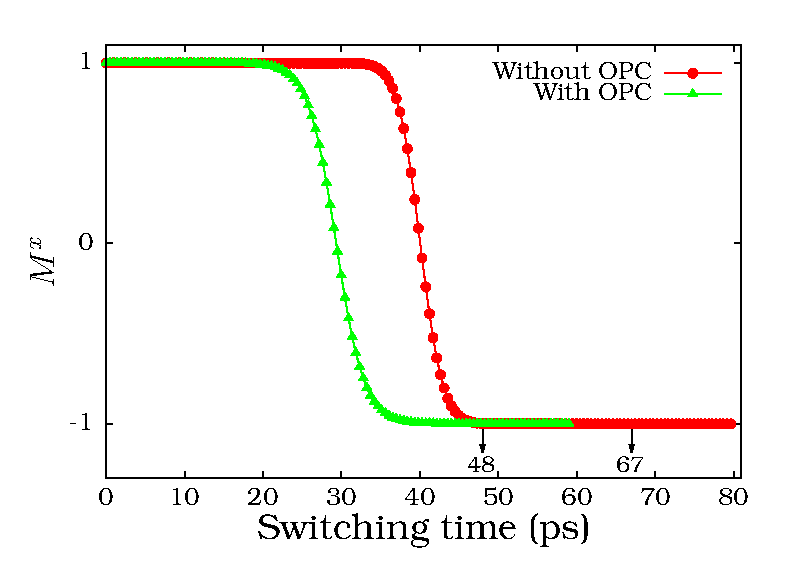
\includegraphics[width=7in]{opc}
\end{tikzfigure}

{\large Fig.2: A plot of magnetization versus switching time for the Co/Cu/NiFe nanopillar in the presence and absence of the orange peel coupling for the applied current density $J=4\times10^{8} A cm^{-2}$. Presence of orange peel coupling reduces the switching time.}
}
%%%%%%%%%%%%%%%%%%%%%%%%%%%%%%%%%%%%%%%%%%%%%%%%%%%%%%%%%%%%%%%%%%%%%%%%%%%%%%%%%%%%%%%%%%%%%%%%%%%%%%%%%%%%%%
% Next Block
\blocknode{Effect of current density}{
\begin{tikzfigure}
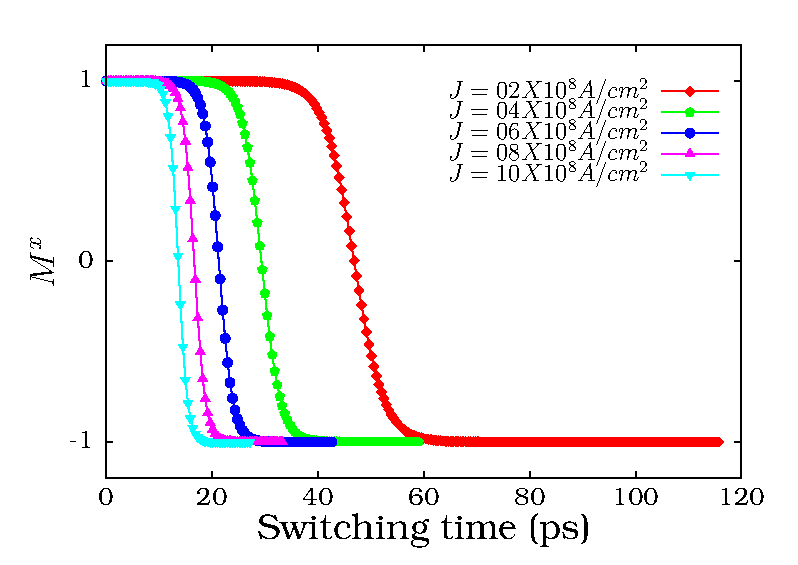
\includegraphics[width=7in]{jvary}
\end{tikzfigure}
{\large Fig.3: A plot of magnetization versus switching time for the Co/Cu/NiFe nanopillar for different current densities. The applied current density increases from $2\times10^{8} A cm^{-2}$ to $10\times10^{8} A cm^{-2}$ in the interval of $2\times10^{8} A cm^{-2}$. Switching time decreases from 78 ps to 23 ps.}
}
%%%%%%%%%%%%%%%%%%%%%%%%%%%%%%%%%%%%%%%%%%%%%%%%%%%%%%%%%%%%%%%%%%%%%%%%%%%%%%%%%%%%%%%%%%%%%%%%%%%%%%%%%%%%%%

%%%%%%%%%%%%%%%%%%%%%%%%%%%%%%%%%%%%%%%%%%%%%%%%%%%%%%%%%%%%%%%%%%%%%%%%%%%%%%%%%%%%%%%%%%%%%%%%%%%%%%%%%%%%%%
% Next Block
\blocknode{Effect of spacer and free layer thicknesses}{
\begin{tikzfigure}
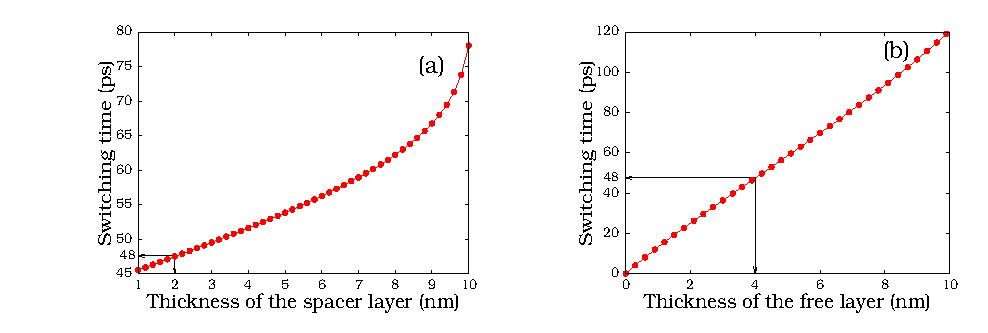
\includegraphics[width=14in]{tsvary_and_dvary}
\end{tikzfigure}
{\large Fig.4: (a). A plot of thickness of the spacer layer versus switching time for the Co/Cu/NiFe nanopillar for the applied current density $J=4\times10^{8} A cm^{-2}$. (b). A plot of thickness of the free layer versus switching time for the Co/Cu/NiFe nanopillar for the applied current density $J=4\times10^{8} A cm^{-2}$.}
}
%%%%%%%%%%%%%%%%%%%%%%%%%%%%%%%%%%%%%%%%%%%%%%%%%%%%%%%%%%%%%%%%%%%%%%%%%%%%%%%%%%%%%%%%%%%%%%%%%%%%%%%%%%%%%%
% Next Block
\blocknode{Conclusions}{
\large
\begin{itemize}
\item The spin current induced magnetization switching dynamics in Co/Cu/NiFe nanopillar with orange peel coupling is studied by solving the governing Landau-Lifshitz-Gilbert- Slonczewski equation numerically.
\item The switching time of the nanopillar device reduces from 67 ps to 48 ps  when there exists the orange peel coupling between the ferromagnetic layers.
\item The switching time decreases, when the thickness of the spacer layer and also the free layer reduces.
\item Thus, We can achieve fast switching by making the free layer and spacer layer in the nanopillar device with  minimal thicknesses.
\end{itemize}
}
\blocknode{References}{
\large
\begin{enumerate}
\item P. Sabareesan and M. Daniel, \emph{Phys. Scr.} {\bf84}, 035706 (2011).
\item J. Zhang, and R. M. White, \emph{IEEE Trans. Magnetics}, {\bf287}, 2000 (1989).
\item L. N$\acute{e}$el, \emph{C. R. Acad. Sci., Paris}, {\bf 255}, 1676 (1962).
\item J. C. S. Kools, W. Kula, D. Mauri and T. Lin, \emph{J. Appl. Phys.}, {\bf 85}, 4466 (1999).
\item D. Aravinthan, P. Sabareesan and M. Daniel, Impact of Orange Peel Coupling on Magnetization Switching in Nanopillar, (Communicated for publication.)
 \end{enumerate}
}
\vspace{1cm}
\plainblock[0]{($(currenty)+(1,1)$)}{35}{$^*$ For Correspondence:}{
{\large \bf \begin{center} E-mail: d.aravinthan@gmail.com\\
Web: www.idaravinthan.info
 \end{center}
}}
\end{tikzpicture}
\end{document}
